\documentclass[a4paper]{article}
\usepackage{graphicx} % Required for inserting images
\usepackage{listings}

\usepackage{pgf-umlcd}
\usepackage[english,ngerman]{babel}
\usepackage[inkscapelatex=false]{svg}
\usepackage{hyperref}
\usepackage{float}
\usepackage{geometry}
\usepackage{titling}


\selectlanguage{ngerman}


\title{
\LARGE{Client/Server Chat Anwendung mit WebSockets}  \\ 
\normalsize{Dokumentation für "Projekt Informatik"}
}
\author{}
\date{März 2024}

\begin{document}


\maketitle




\tableofcontents
\newpage


\section{Einleitung}

Diese Client/Server Chat Anwendung wurde in der Programmiersprache Rust entwickelt. Der Client tritt einem Chat bei, indem er seinen Namen, eine Gruppe und die Serveradresse angibt. Die Gruppe bestimmt, was für Nachrichten dem Client angezeigt werden und ermöglicht eine 'private' Unterhaltung in einer Art Chat-Raum. Der Server verwaltet die Gruppen und leitet Nachrichten an die entsprechenden Clients weiter. Beim Verbinden von einem neuen Client werden alle vorherigen Nachrichten aus der Gruppe an den Client gesendet. Die Kommunikation zwischen Client und Server erfolgt über WebSockets und ist somit im lokalen Netzwerk oder über das Internet möglich.



\subsection{Ausführen}

\begin{figure}[H]
    \centering
    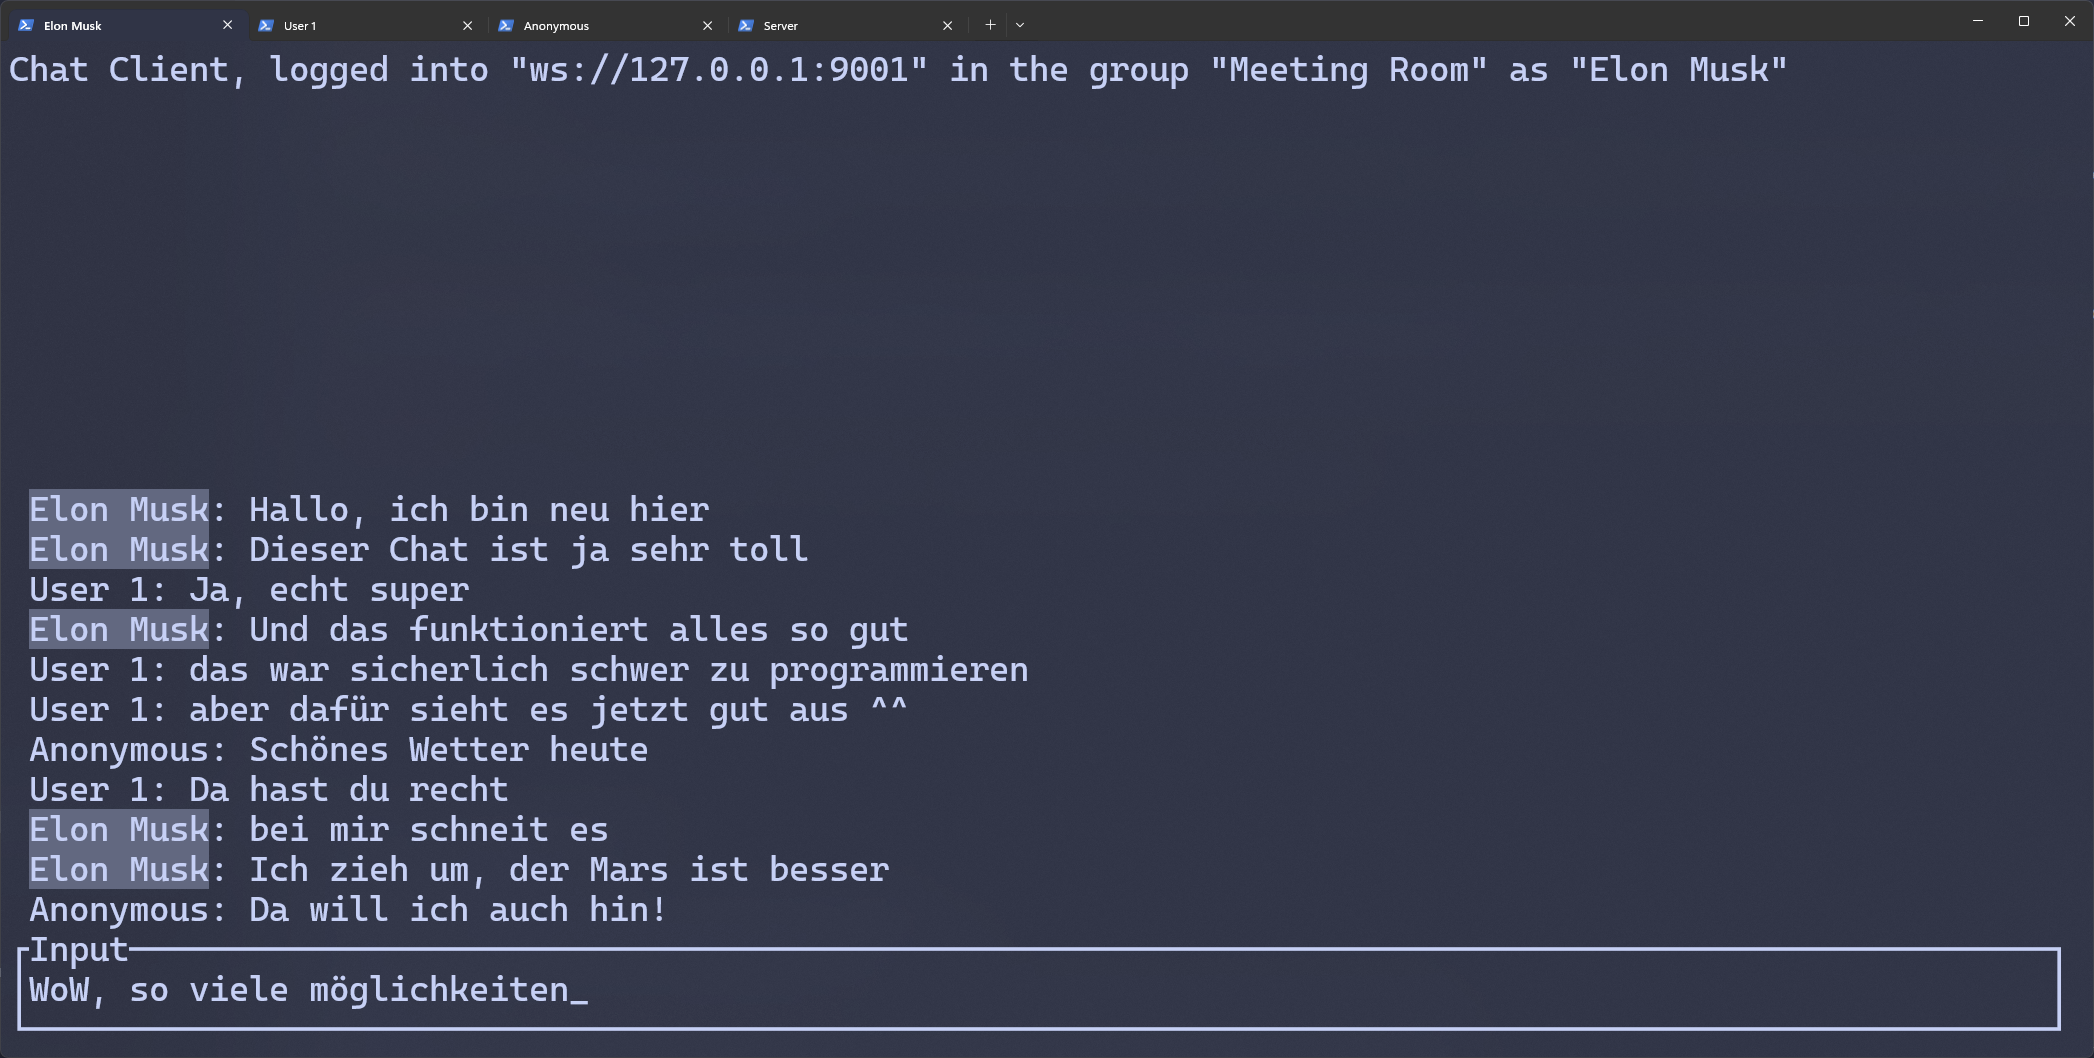
\includegraphics[width=0.9\textwidth]{interface.png}
\end{figure}

Die Binärdateien können direkt ausgeführt werden, ohne irgendwelche Dependencies. Oder das Projekt kann mit \texttt{cargo} kompiliert und ausgeführt werden. Zum Kompilieren wird Rust benötigt, welches auf dieser Seite heruntergeladen werden kann: \url{https://www.rust-lang.org/tools/install}.
\begin{verbatim}    
    // Kompilieren und ausführen
    cargo run --release --bin chat-server
    cargo run --release --bin chat-client

    // Kompilieren
    cargo build --release
    ./target/release/chat-server
    ./target/release/chat-client
\end{verbatim}
Es können auch mehr detailierte Logs aktiviert werden, indem die Umgebungsvariable \texttt{RUST\_LOG} gesetzt wird.
\begin{verbatim}
    RUST_LOG=debug cargo run --release --bin chat-server 
\end{verbatim}
oder die logs können ausgeschaltet werden
\begin{verbatim}
    RUST_LOG=off ./target/release/chat-client
\end{verbatim}


\newpage
\subsection{Protokoll}

\begin{figure}[H]
    \centering
    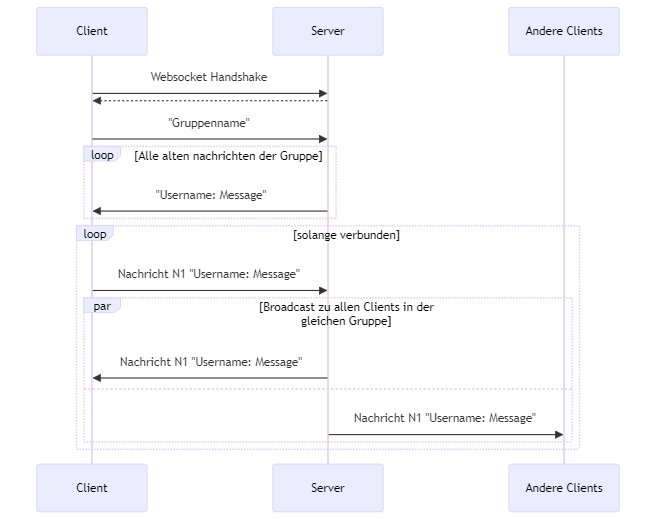
\includegraphics[width=0.70\textwidth]{protocol2.png}
    \caption{Das Protokoll}\label{fig:protocol}
\end{figure}

Der Client baut eine WebSocket-Verbindung zum Server auf und sendet einen Handshake. Danach wählt der Client eine Gruppe und sendet eine Nachricht an den Server.
Der Server sendet alle gespeicherten Nachrichten in der Gruppe an den Client. Wenn der Server eine Nachricht von einem Client empfängt, leitet er diese an alle anderen Clients in der Gruppe weiter.


\subsection{Bibliotheken}

Das Projekt verwendet die folgenden Bibliotheken:

\begin{itemize}
    \setlength\itemsep{0em}
    \item \texttt{tokio} für asynchrone Operationen und Multithreading
    \item \texttt{tokio-tungstenite} für die WebSocket-Kommunikation
    \item \texttt{sqlx} für die Datenbankanbindung
    \item \texttt{ratatui} für die Benutzerschnittstelle
    \item \texttt{crossterm} für die Eingabeverarbeitung
    \item \texttt{env\_logger} für das Logging
\end{itemize}

\newpage

\section{Client}

\subsection{main.rs}

Die Datei \texttt{main.rs} enthält die Hauptfunktion des Chat-Clients. Sie startet die Anwendung, initialisiert den Logger, erfasst den Benutzernamen, die Gruppe und die Serveradresse über die Standardeingabe und führt die Anwendung aus. Wenn die Anwendung die Verbindung zum Server verliert, wird eine Fehlermeldung ausgegeben.

\subsection{app.rs}

Die \texttt{Application}-Klasse ist verantwortlich für die Verwaltung der Anwendung, die WebSocket-Kommunikation, die Benutzerschnittstelle und das Modell. Sie enthält Informationen über die URL des Websockets, den Benutzernamen, die Gruppe, die Eingabeverarbeitung, die Benutzerschnittstelle (TUI), das Datenmodell und den WebSocket.


\subsection{input.rs}

Die Datei \texttt{input.rs} implementiert die \texttt{EventHandler}-Klasse, die für die Verarbeitung von Eingabe Events im Terminal zuständig ist.
Die \texttt{EventHandler}-Klasse erstellt einen Kanal (\texttt{mpsc}), um Ereignisse an den Hauptthread zu senden, und startet einen Thread, um Ereignisse aus dem Terminal zu lesen. Dieser Thread verarbeitet Tastatureingaben und gibt entsprechende Ereignisse zurück, wie z.B. \texttt{Quit}, \texttt{Send}, \texttt{Backspace}, \texttt{Resize}, \texttt{Refresh},  und \texttt{Input}. Die \texttt{next}-Methode wartet auf das nächste Ereignis und gibt es zurück.


\subsection{model.rs und tui.rs}

\begin{figure}[hbt]
    \centering
    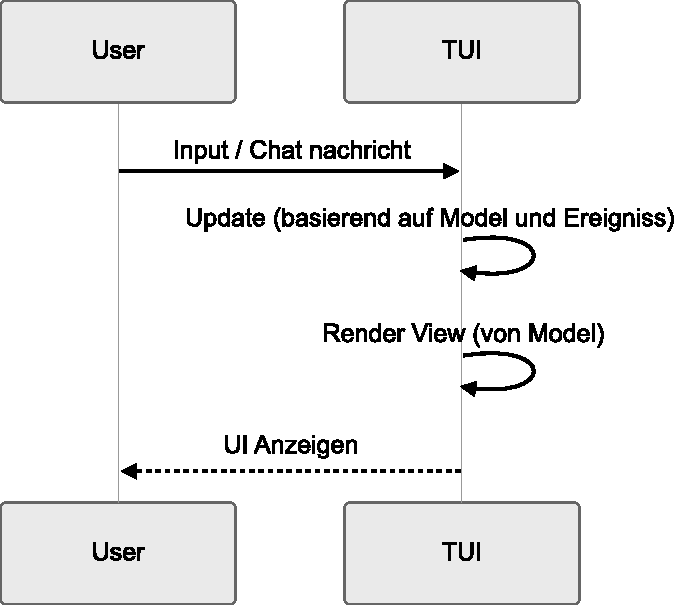
\includegraphics[width=0.5\textwidth]{ELM.pdf}
    \caption{Die Elm Architektur}\label{fig:elm}
\end{figure}

Die \texttt{Model}-Klasse entspricht dem Modell in der Elm-Architektur. Sie speichert Informationen über die URL des Websockets, den Benutzernamen, die aktuelle Eingabe im Textbereich, die Gruppe und die empfangenen Nachrichten. Ähnlich wie in Elm wird das Modell als einziger, unveränderbarer Zustand betrachtet, der die gesamte Anwendungsdaten enthält.

Die \texttt{ChatMessage}-Klasse repräsentiert eine einzelne Chat-Nachricht und implementiert Methoden zum Serialisieren und Deserialisieren.

Die \texttt{TUI}-Klasse ist für das Rendering der Benutzerschnittstelle verantwortlich. Sie verwendet die \texttt{ratatui}-Bibliothek, um Textelemente und Widgets anzuzeigen. Ähnlich wie in Elm wird die Benutzerschnittstelle in einem funktionalen Stil gerendert, wobei die render-Methode die Darstellung des aktuellen Modells auf dem Bildschirm steuert.


\subsection{websocket.rs} \label{ws_client}

Die Klasse \texttt{Websocket} repräsentiert eine WebSocket-Verbindung. Sie enthält Kanäle zum Lesen und Schreiben von Nachrichten mit asynchronem Code. Sobald eine neue Nachricht empfangen wird, wird diese über einen Kanal an den Hauptthread gesendet mithilfe der \texttt{receive}-Methode. Das Senden von Nachrichten erfolgt in einem separaten Thread.


\section{Server}


\subsection{main.rs}

Die Datei \texttt{main.rs} enthält die Hauptfunktion des Chat-Servers. Sie initialisiert die Anwendung, konfiguriert das Logging und fragt den Benutzer nach dem Server-Port. Falls der Benutzer keinen Port eingibt, wird der Standardport '9001' verwendet.

\subsection{app.rs}



Die Datei \texttt{app.rs} enthält die Implementierung der Anwendungslogik für den Chat-Server. Sie definiert die Klasse \texttt{Application}, die die zentrale Anwendung darstellt. Diese Klasse verwaltet die Verbindungen zu Clients, die Datenbankverbindung und koordiniert die Kommunikation zwischen den Clients über WebSockets.

\begin{itemize}
    \item Die Klasse \texttt{Application} enthält Felder für die Serveradresse (\texttt{address}), die Verbindungen zu den Clients (\texttt{connections}) und die Datenbankverbindung (\texttt{db}).
    \item Die Methode \texttt{new} erstellt eine neue Anwendungsinstanz mit der angegebenen Serveradresse.
    \item Die Methode \texttt{run} führt die Anwendungslogik aus, indem sie eine Verbindung zur Datenbank herstellt, WebSocket-Verbindungen akzeptiert und eingehende Nachrichten von den Clients verarbeitet.
    \item Die Methode \texttt{on\_connection} wird aufgerufen, wenn eine neue Verbindung zu einem Client hergestellt wird. Sie behandelt das Lesen und Senden von Nachrichten sowie das Speichern von Nachrichten in der Datenbank.
\end{itemize}

\subsection{connection.rs}

Wandelt eine WebSocket-Verbindung um in eine \texttt{Connection}-Klasse, die sicherstellt, dass dem Protokoll in der Abbildung \ref{fig:protocol} gefolgt wird.

\subsection{websocket.rs}

Siehe: \ref{ws_client} Client \texttt{websocket.rs}


\subsection{database.rs}


\begin{verbatim}
    CREATE TABLE IF NOT EXISTS messages (
        id INTEGER PRIMARY KEY,
        group_name TEXT NOT NULL,
        username TEXT NOT NULL,
        message TEXT NOT NULL
    )
\end{verbatim}


Die Datei \texttt{database.rs} enthält Funktionen zur Verwaltung der SQLite-Datenbank.




\begin{itemize}
    \item Die Funktion \texttt{establish\_connection} erstellt eine Verbindung zur SQLite-Datenbank, die von mehreren Threads geteilt werden kann.
    \item Die Funktion \texttt{insert\_message} fügt eine neue Nachricht in die Datenbank ein.
    \item Die Funktion \texttt{get\_messages} ruft Nachrichten aus der Datenbank ab, die einer bestimmten Gruppe zugeordnet sind.
\end{itemize}


\end{document}
